\documentclass{standalone}

\usepackage[english]{babel}

% to use colors

\usepackage{xcolor}

% to define font size

\usepackage{ulem}
\usepackage{moresize}
\usepackage{anyfontsize}

% to use tikz and its libraries

\usepackage{tikz-timing}
\usepackage{tikz}

\usetikzlibrary{backgrounds}
\usetikzlibrary{decorations.pathreplacing, positioning, calc, arrows, shapes, automata, petri, patterns,decorations.markings}

% to use tikzmark, to place and refer to marks outside the current figure

\tikzset{every picture/.style={remember picture}}

% styles for transitions

\tikzset{transition/.append style={fill=black!20, thick}}
\tikzset{transition/.append style={fill=black!20, thick}}

% styles for test and inhib arcs.

\tikzstyle{test}=[pre, *-]
\tikzstyle{inhib}=[pre, o-]

% Arrow positioning in a path

\tikzset{->-/.style={decoration={
  markings,
  mark=at position #1 with {\arrow{>}}},postaction={decorate}}}

\tikzset{-<-/.style={decoration={
  markings,
  mark=at position #1 with {\arrow{<}}},postaction={decorate}}}

%%%%%%%%%%%%%%%%%%%%%%%%%%%%%%%%%%%%%%%%%%%%%%%%%%
%                  BEGIN DOCUMENT                %
%%%%%%%%%%%%%%%%%%%%%%%%%%%%%%%%%%%%%%%%%%%%%%%%%%

\begin{document}

\begin{tikzpicture}
  
  \node (pn) {
    \begin{tikzpicture}[remember picture]
      
      \node[place] (p0) {};
      \node (pzLabel) at ($(p0)-(.7,0)$) {$p_0$};
      
      \node[transition] (t0) at ($(p0)-(0,1)$) {};
      \node (tzLabel) at ($(t0)-(.5,0)$) {$t_0$};
      
      \node[place] (p1) at ($(t0)-(0,1)$) {};
      \node (poLabel) at ($(p1)-(.7,0)$) {$p_1$};

      \draw (p0) edge[post] (t0);
      \draw (t0) edge[post] (p1);

    \end{tikzpicture}
  };

  \node[draw, rectangle, inner sep=2mm] (vhdl) at ($(pn.east)+(3,0)$) {
    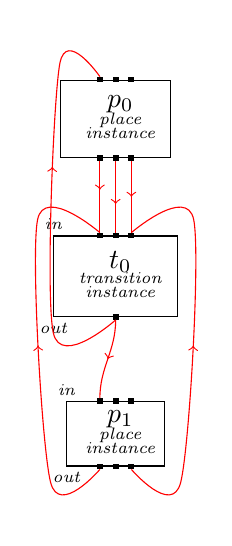
\begin{tikzpicture}[remember picture]

      \node (cl) at (0,0) {};
      \node (cr) at (2,0) {};
      
      % P0 Component + I/O
      \node[draw, black, inner sep=2mm] at ($(cl)!.5!(cr)$) (compP0) {        
        \renewcommand{\arraystretch}{.3}
        \begin{tabular}{@{}c@{}}
          $p_0$ \\
          \ssmall\it place \\
          \ssmall\it instance \\
        \end{tabular}
      };

      % \node[anchor=south west] at ($(compP0.north west)$) {\ssmall\itshape in};
      \node[draw, black, fill=black, inner sep=.3mm] (clkP0) at ($(compP0.north)-(.2,0)$) {};
      \node[draw, black, fill=black, inner sep=.3mm] (compP0In1) at (compP0.north) {};
      \node[draw, black, fill=black, inner sep=.3mm] (compP0In2)  at ($(compP0.north)+(.2,0)$) {};

      % \node at ($(compP0.south west)-(0,4pt)$) {\ssmall\itshape out};
      \node[draw, black, fill=black, inner sep=.3mm] (compP0Out0) at ($(compP0.south)-(.2,0)$) {};
      \node[draw, black, fill=black, inner sep=.3mm] (compP0Out1) at (compP0.south) {};
      \node[draw, black, fill=black, inner sep=.3mm] (compP0Out2) at ($(compP0.south)+(.2,0)$) {};

      % T0 Component + I/O
      
      \node[draw, black, inner sep=2mm] (compT0) at ($(compP0)-(0,2)$) {
        \renewcommand{\arraystretch}{.3}
        \begin{tabular}{@{}c@{}}
          $t_0$ \\
          \ssmall\it transition \\
          \ssmall\it instance \\
        \end{tabular}
      };

      \node at ($(compT0.north west)+(0,4pt)$) {\ssmall\itshape in};
      \node[draw, black, fill=black, inner sep=.3mm] (clkT0) at ($(compT0.north)-(.2,0)$) {};
      \node[draw, black, fill=black, inner sep=.3mm] (compT0In1) at (compT0.north) {};
      \node[draw, black, fill=black, inner sep=.3mm] (compT0In2) at ($(compT0.north)+(.2,0)$) {};

      \node at ($(compT0.south west)-(0,4pt)$) {\ssmall\itshape out};
      \node[draw, black, fill=black, inner sep=.3mm] (compT0Out1) at (compT0.south) {};

      % P1 Component + I/O
      
      \node[draw, black] (compP1) at ($(compT0)-(0,2)$) {
        \renewcommand{\arraystretch}{.3}
        \begin{tabular}{@{}c@{}}
          $p_1$ \\
          \ssmall\it place \\
          \ssmall\it instance \\
        \end{tabular}
      };

      \node at ($(compP1.north west)-(0,-4pt)$) {\ssmall\itshape in};
      \node[draw, black, fill=black, inner sep=.3mm] (clkP1) at ($(compP1.north)-(.2,0)$) {};
      \node[draw, black, fill=black, inner sep=.3mm] (compP1In1) at (compP1.north) {};
      \node[draw, black, fill=black, inner sep=.3mm] (compP1In2) at ($(compP1.north)+(.2,0)$) {};

      \node at ($(compP1.south west)-(0,4pt)$) {\ssmall\itshape out};
      \node[draw, black, fill=black, inner sep=.3mm] (compP1Out0) at ($(compP1.south)-(.2,0)$) {};
      \node[draw, black, fill=black, inner sep=.3mm] (compP1Out1) at (compP1.south) {};
      \node[draw, black, fill=black, inner sep=.3mm] (compP1Out2) at ($(compP1.south)+(.2,0)$) {};

      % Interconnections
      
      \draw ($(compP0Out0.south)$) edge[red,->-=.4] ($(clkT0.north)$);
      \draw ($(compP0Out1.south)$) edge[red,->-=.6] ($(compT0In1.north)$);
      \draw ($(compP0Out2.south)$) edge[red,->-=.5] ($(compT0In2.north)$);

      \draw ($(compT0Out1.south)$) edge[red,->-=.5,in=90,out=-90] ($(clkP1.north)$);
      \draw[red,->-=.6] plot [smooth,tension=.5] coordinates { (compT0Out1.south)
        ($(compT0.south west)-(0,.2)$) ($(compP0.north west)+(0,.2)$) (clkP0.north)};

      \draw[red,->-=.5] plot [smooth,tension=.5] coordinates { (compP1Out0.south)
        ($(compP1.south west)-(.2,.2)$) ($(compT0.north west)+(-.2,.2)$) (clkT0.north)};

      \draw[red,->-=.5] plot [smooth,tension=.5] coordinates { (compP1Out2.south)
        ($(compP1.south east)+(.2,-.2)$) ($(compT0.north east)+(.2,.2)$) (compT0In2.north)};
    \end{tikzpicture}
  };

  \node at ($(vhdl.north west)+(0,6pt)$) {\itshape in};
  \node[draw, black, fill=black, inner sep=.5mm] (clkVhdl) at ($(vhdl.north west)+(.4,0)$) {};
  \node[draw, black, fill=black, inner sep=.5mm] at ($(vhdl.north west)+(.8,0)$) {};
  \node[draw, black, fill=black, inner sep=.5mm] at (vhdl.north) {};
  \node[draw, black, fill=black, inner sep=.5mm] at ($(vhdl.north east)-(.8,0)$) {};
  \node[draw, black, fill=black, inner sep=.5mm] at ($(vhdl.north east)-(.4,0)$) {};
  
  \node at ($(vhdl.south west)-(3pt,6pt)$) {\itshape out};
  \node[draw, black, fill=black, inner sep=.5mm] at ($(vhdl.south west)+(.4,0)$) {};
  \node[draw, black, fill=black, inner sep=.5mm] at ($(vhdl.south west)+(.8,0)$) {};
  \node[draw, black, fill=black, inner sep=.5mm] at (vhdl.south) {};
  \node[draw, black, fill=black, inner sep=.5mm] at ($(vhdl.south east)-(.8,0)$) {};
  \node[draw, black, fill=black, inner sep=.5mm] at ($(vhdl.south east)-(.4,0)$) {};
  
  \node[draw, black, inner sep=1mm] (placeBeh) at ($(vhdl.east)+(2,1)$) {
    \renewcommand{\arraystretch}{.5}
    \begin{tabular}{@{}c@{}}
      Place\\
      design \\
      \ssmall(interface + behavior) \\
    \end{tabular}
  };
  
  \node[draw, black, inner sep=1mm] (transitionBeh) at ($(vhdl.east)+(2,-1)$) {
    \renewcommand{\arraystretch}{.5}
    \begin{tabular}{@{}c@{}}
      Transition\\
      design \\
      \ssmall(interface + behavior) \\
    \end{tabular}
  };

  \draw[decorate, red, decoration={brace, amplitude=3pt, raise=6pt}]
  ($(placeBeh.north west)$) -- ($(placeBeh.north east)$);
  
  \node[anchor=south, yshift=4mm] at ($(placeBeh.north west)!.5!(placeBeh.north east)$) {
    \textcolor{red}{Static}
  };

  % EDGES
  \draw (compP0.east) edge[->, thick, dotted,out=0,in=180] ($(placeBeh.west)+(0,.2)$);
  \draw (compT0.east) edge[->, thick, dotted,out=0,in=180] ($(transitionBeh.west)$);
  \draw (compP1.east) edge[->, thick, dotted,out=0,in=180] ($(placeBeh.west)-(0,.2)$);
  
  % \node (clk) at ($(p0.north)+(0,10pt)$) {\ssmall \texttt{Clock signal}
  %   % 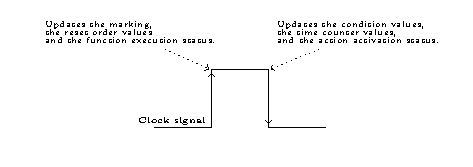
\includegraphics[keepaspectratio,width=.25\linewidth]{sync-exec}
  % };

  \draw[decorate, blue, decoration={brace, amplitude=3pt, raise=6pt}]
  ($(vhdl.north west)+(0,.3)$) -- ($(vhdl.north east)+(0,.3)$);
  
  \node[anchor=south, yshift=4mm] at ($(vhdl.north west)!.5!(vhdl.north east)+(0,.3)$){
    \textcolor{blue}{Generated} };
  
  % Clk signal connections

  % \draw($(clk.east)$) -| ($(clkP1.north)-(13pt,-3pt)$) -| ($(clkP1.north)$);
  % \draw ($(clkP0.north)-(13pt,-3pt)$) -| ($(clkP0.north)$);
  % \draw ($(clkT0.north)-(13pt,-3pt)$) -| ($(clkT0.north)$);
  
  \draw (pn.east)
  edge[double, ->, thick]
  % node[yshift=1em] {Transformation}
  ($(vhdl.west)-(.4,0)$);
  
\end{tikzpicture}

\end{document}